\documentclass[Arkitektur/System_main.tex]{subfiles}
\begin{document}
\subsubsection{Applikationsmodel for Bolddispenser} \label{sec:balldispenser_application_model}
I dette afsnit præsenteres applikationsmodellen for bolddispenseren, hvor der er lavet et overordnet klassediagram og statemachine for dispenseren, som spiller sammen med et sekvensdiagram for UC1 og UC4, der var de mest relevante i forbindelse med Bolddispenser.

\textbf{Klassediagram: Bolddispenser}\\
Startes der med klassediagrammet for det overordnede overblik over relationer og metoder, så ses dette i figur \ref{fig:cd_balldispenser}. I figuren ses relationer og metoder for alle de relevante use cases i forhold til bolddispenseren.
\begin{figure}[H]
    \centering
    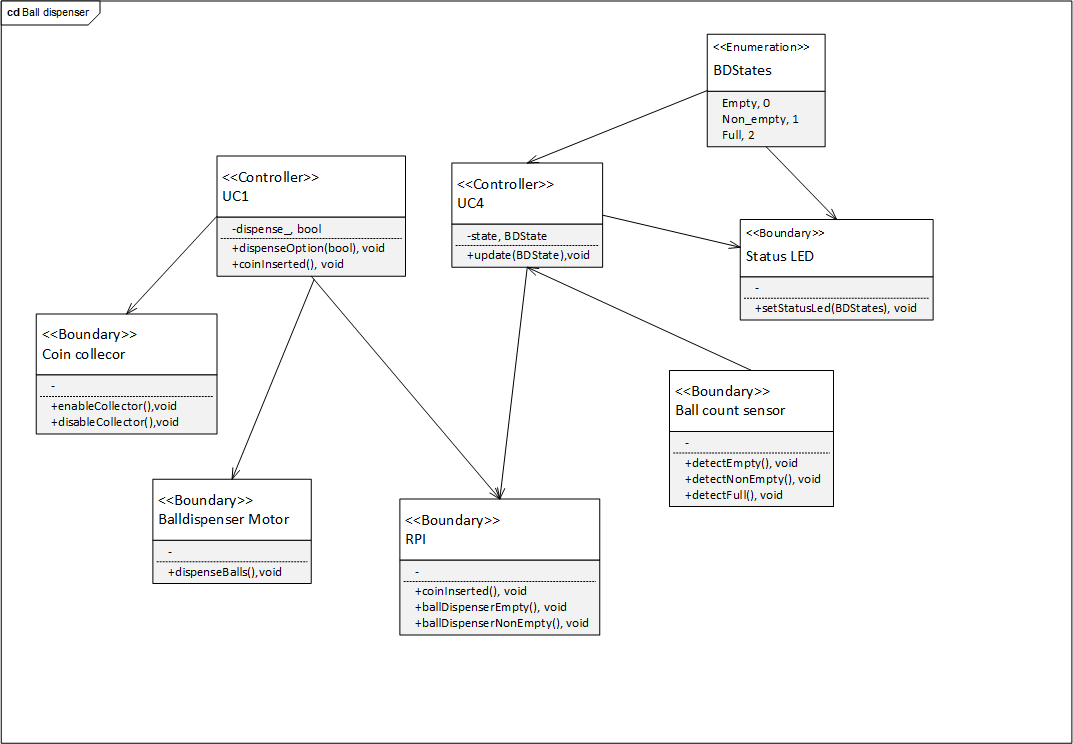
\includegraphics[width=\textwidth]{Arkitektur/Softwarearkitektur/Applikationsmodel/BallDispenser/graphicsBallDispenser/ApplikationsmodelBolddispensercd.png}
    \caption{Class Diagram for bolddispenser}
    \label{fig:cd_balldispenser}
\end{figure}
\newpage

\textbf{Tilstandsmaskine: Bolddispenser}\label{sec:BallDispSTM}\\
I bolddispenseren kan der deles op i to forskellige typer tilstande. En tilstand om bolddispenserens kapacitet af bolde og en tilstand om bolddispenseren må dispensere bolde. Hvordan bolddispenseren bevæger sig imellem disse tilstande, og hvad der sker kan ses i figur \ref{fig:stm_balldispenser}. 
Af figuren ses det at den øverste del af statemachine diagrammet er det, der omhandler kapacitet af boldene. Der er ikke nogen state, som bolddispenseren skal starte i, idet bolddispenseren kan være i alle states ved opstart. Ved eksekvering af UC4, starter den dog ud i empty, da dette er en prækondition til udførelsen af use casen. 
Når der så fyldes bolde på bolddispenseren kan den altså gå fra empty til Nonempty i det en sensor detektere at minimumsgrænsen for bolde er nået. Dette trigger en opdatering af status led'erne (Der indikere om der mangler bolde), samt en opdatering på RPi, idet den skal vide om et nyt spil kan påbegyndes. 
Hvis påfyldning så fortsættes, så vil boldene til sidst opbruge alt pladsen, hvilket igen trigger en opdatering, men denne gang kun af status led'en (Det har ingen betydning for RPi, om bolddispenseren er fuld).
\begin{figure}[H]
    \centering
    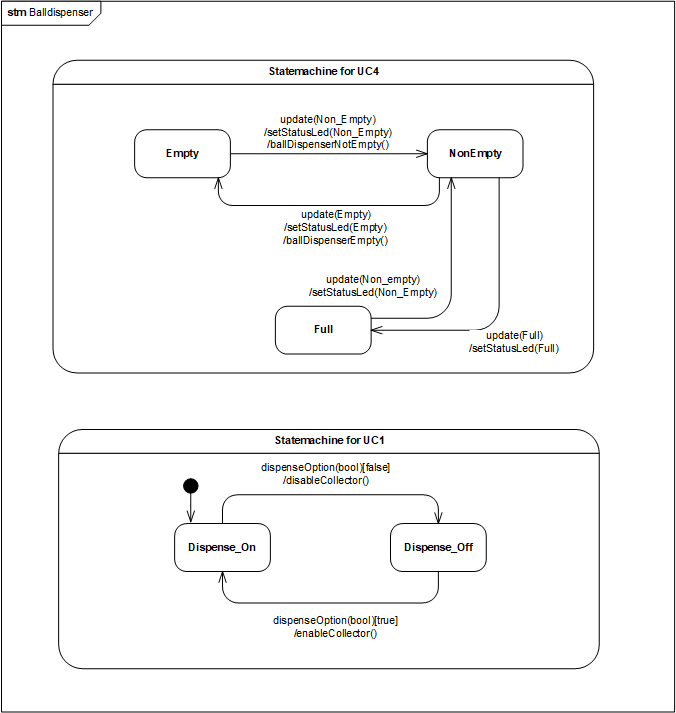
\includegraphics[width=\textwidth]{Arkitektur/Softwarearkitektur/Applikationsmodel/BallDispenser/graphicsBallDispenser/ApplikationsmodelBolddispenserstm.PNG}
    \caption{Tilstandsmaskine for bolddispenser}
    \label{fig:stm_balldispenser}
\end{figure}
\newpage

\textbf{Sekvensdiagram UC1: Bolddispenser}\\
Når et spil skal startes, er det i pricippet bolddispenserens ansvar at starte spillet i det, den skal registrere indsættelsen af en mønt og sende et signal om dette til RPI'en. Forløbet i dette er beskrevet i figur \ref{fig:seq_uc1_balldispenser}.
\begin{figure}[H]
    \centering
    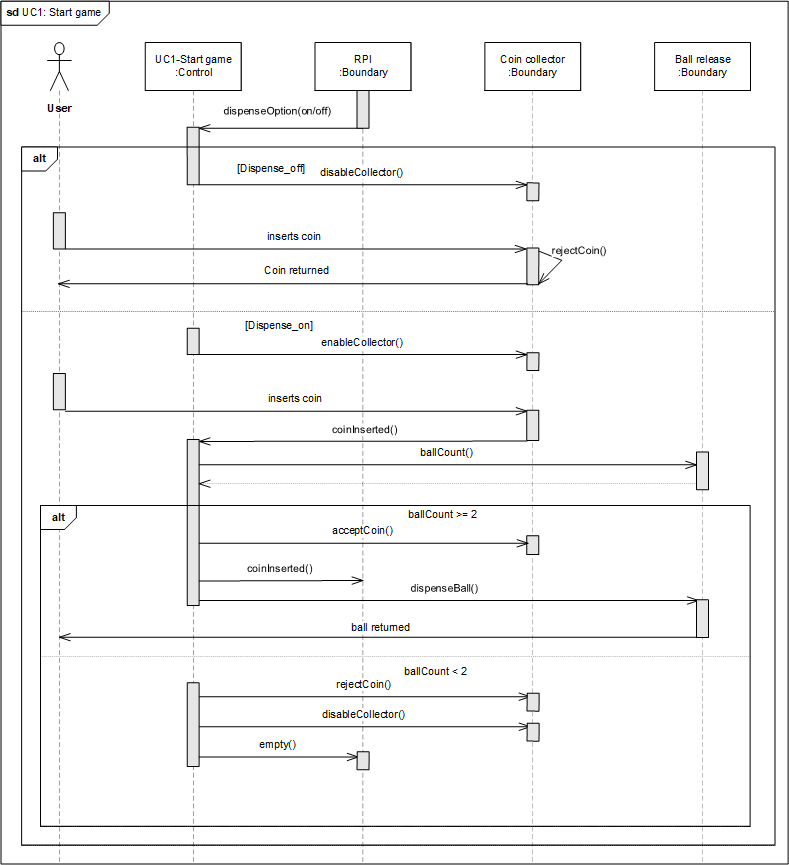
\includegraphics[width=\textwidth]{Arkitektur/Softwarearkitektur/Applikationsmodel/BallDispenser/graphicsBallDispenser/sdUC1.png}
    \caption{Sekvensdiagram for UC1 for bolddispenser}
    \label{fig:seq_uc1_balldispenser}
\end{figure}
\newpage

\textbf{Sekvensdiagram UC4: Bolddispenser}\\
Når der skal udøves service på bolddispenseren, kan dette også beskrives i applikationen som forløbet, der ses i figur \ref{fig:seq_uc4_balldispenser}.
\begin{figure}[H]
    \centering
    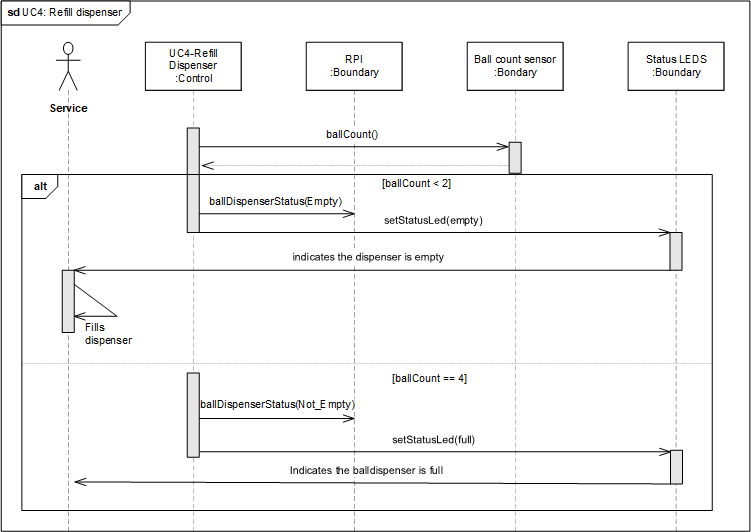
\includegraphics[width=\textwidth]{Arkitektur/Softwarearkitektur/Applikationsmodel/BallDispenser/graphicsBallDispenser/sdUC4.png}
    \caption{Sekvensdiagram for UC4 for bolddispenser}
    \label{fig:seq_uc4_balldispenser}
\end{figure}
\newpage
{\large\textbf{Funktionsbeskrivelser: CoinDispenser Controller}}\\[0.2cm]
\textbf {coinInserted(): void}
\begin{adjustwidth}{1cm}{0pt}
\textbf {Beskrivelse:} Denne funksjonen er hoved kontrol funksjonen til ball dispenser. Den blir kalt hver gang det skjer en coin detection. Den starter all logiken som skjer i UC1 \\ [0.2cm]
\textbf {Parametere:} ingen \\ [0.2cm]
\textbf {Returneringsverdi:} ingen \\ [0.2cm]
\end{adjustwidth}

\textbf {sendToRPi(uint8\_t message): void}
\begin{adjustwidth}{1cm}{0pt}
\textbf {Beskrivelse:} Denne funksjonen sender en melding til RPien via I2C protokollen. \\ [0.2cm]
\textbf {Parametere:} 
\begin{itemize}
    \item Message: Beskjeden som skal sendes til RPien, de spesifikke beskjedene kan sees i Grenseflater avsnittet (\ref{sec:protocols})
\end{itemize}
\\ [0.2cm]
\textbf {Returneringsverdi:} ingen \\ [0.2cm]
\end{adjustwidth}

\textbf {handleI2CData: void}
\begin{adjustwidth}{1cm}{0pt}
\textbf {Beskrivelse:} Denne funksjonen ligger i main som konstant looper til dataen i writebuffer blir endret hvor den så kaller enable eller disable dispenser.  \\ [0.2cm]
\textbf {Parametere:} \\ [0.2cm]
\textbf {Returneringsverdi:} ingen \\ [0.2cm]
\end{adjustwidth}

{\large\textbf{Funktionsbeskrivelser: CoinDespenser}}\\[0.2cm]

\textbf {handleCoin: void}
\begin{adjustwidth}{1cm}{0pt}
\textbf {Beskrivelse:} Denne funksjonen er kontroll funskjonen til coinDispenser, den kaller den riktige funksjonen i forhold til om den er enabled eller disabled stadiet. \\ [0.2cm]
\textbf {Parametere:} ingen \\ [0.2cm]
\textbf {Returneringsverdi:} ingen \\ [0.2cm]
\end{adjustwidth}


\textbf {rejectCoin: void}
\begin{adjustwidth}{1cm}{0pt}
\textbf {Beskrivelse:} Denne funksjonen er ansvarlig for myntavvisning, den kaller de kontrollfunksjonene som kreves for å avvise en mynt fra systemet, og gjenaktiverer deteksjons-ISR-en for å gjøre systemet klar for en ny mynt. \\ [0.2cm]
\textbf {Parametere:} ingen \\ [0.2cm]
\textbf {Returneringsverdi:} ingen \\ [0.2cm]
\end{adjustwidth}

\textbf {acceptCoin: void}
\begin{adjustwidth}{1cm}{0pt}
\textbf {Beskrivelse:} Denne funksjonen er ansvarlig for å akseptere en mynt i systemet, det kaller motorstyringsfunksjonene som kreves for å akseptere en mynt, og gjenaktiverer deteksjons-ISR-en for å gjøre systemet klar for en ny mynt. \\ [0.2cm]
\textbf {Parametere:} ingen \\ [0.2cm]
\textbf {Returneringsverdi:} ingen \\ [0.2cm]
\end{adjustwidth}

\textbf {disableDispencer: void}
\begin{adjustwidth}{1cm}{0pt}
\textbf {Beskrivelse:} Denne funksjonen deaktiverer dispenseren, denne funksjonen kalles fra I2C-handleren når den mottar en melding fra GameController at spillet er aktivt. \\ [0.2cm]
\textbf {Parametere:} ingen \\ [0.2cm]
\textbf {Returneringsverdi:} ingen \\ [0.2cm]
\end{adjustwidth}

\textbf {enableDispencer: void}
\begin{adjustwidth}{1cm}{0pt}
\textbf {Beskrivelse:} Denne funksjonen aktiverer dispenseren, denne funksjonen kalles fra I2C-håndtereren når den mottar en melding fra GameController at spillet er inaktivt. \\ [0.2cm]
\textbf {Parametere:} ingen \\ [0.2cm]
\textbf {Returneringsverdi:} ingen \\ [0.2cm]
\end{adjustwidth}


\textbf {enableDispencer: void}
\begin{adjustwidth}{1cm}{0pt}
\textbf {Beskrivelse:} Denne funksjonen clearer og reaktiverer ISRen \\ [0.2cm]
\textbf {Parametere:} ingen \\ [0.2cm]
\textbf {Returneringsverdi:} ingen \\ [0.2cm]
\end{adjustwidth}

\end{document}